We apply a data-driven method~\cite{dyestnote} to estimate the $\dyll$
contributions in the same flavor $\ell^+\ell^-$ final states.
The expected contributions from $\dyll$ events outside the $Z$-mass
region in data can be estimated by counting the number of events near
the $Z$ mass region in data, subtracting from it the non-$Z$
contributions, and scaling it by a ratio $R_{out/in}$ defined as the
fraction of events outside and inside the $Z$-mass region in the
simulation. The $Z$-mass region is selected to be within 7.5 \GeV\, of 
the nominal $Z$ mass. The tight window is chosen to reduce the non-$Z$ 
contributions from top and multi-boson backgrounds. 
The non-$Z$ contributions close to the $Z$-mass region in
data is estimated from the number of events in the $e^\pm\mu^\mp$
final state $N_{in}^{e\mu}$, applying a correction factor that
normalizes the electron-to-muon efficiency $k_{ee/\mu\mu}$. 
$R_{out/in}$ can be obtained both from simulation and
data.  In simulation it is defined as the ratio
$N_{out}^{MC}/N_{in}^{MC}$. 

This method is described mathematically as:
%%%%%%%%%%%%%%%%%%%%%%%%%%%%%%
\begin{eqnarray}
N_{out}^{ll,exp} = R_{out/in}^{ll}(N_{in}^{ll} - 0.5N_{in}^{e\mu}k_{ll}), 
\label{eq:dyest}
\end{eqnarray}
%%%%%%%%%%%%%%%%%%%%%%%%%%%%%%
where $k_{ee} = \sqrt{\frac{N_{in}^{ee,loose}}{N_{in}^{\mu\mu,loose}}}$ for 
$\dyee$ and $k_{mm} = \sqrt{\frac{N_{in}^{\mu\mu,loose}}{N_{in}^{ee,loose}}}$ 
for $\dymm$. In the $k_{ll}$ calcualtion, we apply a loose $\met$ cut on 
minMET of 20 GeV. 

The ZZ/ZW processes contribute to the events in the control region 
of the $m_{\ell\ell}$ region dominated by the DY. 
The contribution from ZZ/ZW becomes comparable to the Drell-Yan background 
after a tight projected \met selection in the same flavor final states. 
The ZZ/ZW events contain natural \met, for which
the detector simulation is reliable\footnote{The ZZ/ZW events with
no \met are suppressed by the same large factor as the DY ones, and
therefore their contribution is as negligible at the level of the
final selection as it would be in the yield at the Z peak without \met
requirement.}. 
We subtract the expected peaking ZZ/ZW
contribution to the yield in the Z peak using the simulation in the 
estimation of number of events within the $Z$ window in data:
%%%%%%%%%%
\begin{equation}\label{eq:dyExtrapM3}
  N(\ell\ell)_{\textrm{signal}} ^{\textrm{DY}}=
  (N(\ell\ell)_{\textrm{control}}^{\textrm{data}}-0.5\times
  N(e\mu)_{\textrm{control}} ^{\textrm{data}}\times k_{\ell\ell}
  -N_{\textrm{control}}^{\textrm{ZV, sim.}} )  \times
  R(\ell\ell)_{out/in}^{DY}
\end{equation}
%%%%%%%%%%%%
The ZZ/ZW contribution in the same flavor final states is then 
taken directly from simulation. 
Seperating the Drell-Yan and ZZ/WZ components 
accounts for the fact that the extrapolation from control 
region to signal region can be different for the two processes when
considering the full Higgs selection. We assume an overall 10\%
uncertainty on the ZZ/ZW yield in the peak, which is anyway
overshadowed by the statistical uncertainty on the observed events in
the Z peak in data.

This $\dyll$ estimation method relies on the assumption that
the dependence of the ratio $R_{out/in}$ on the $\met$ cut is well
modelled by simulation and is relatively flat. 
The variations in the $R_{out/in}$ in different $\met$ regions are assigned as systematics. 
The $\met$ regions considered are [20, 25], [25-30], [30-37] and [37, above]. 
As we do not see any statistically difference between the ee and $\mu\mu$ final states,
 we combine the two final states to gain statistical stability.

We cross-checked the $R_{out/in}$ value in data as well. Background processes
contribute equally to $ee$, $e\mu$, $\mu e$ and $\mu\mu$ final states
(after efficiency corrections), while Drell-Yan only contributes to
$ee$ and $\mu\mu$. Therefore we can subtract $e\mu$ and $\mu e$
contribtutions from $ee$ and $\mu\mu$ ones to get an estimate of
Drell-Yan. We have found good agreement between data and MC in the 
Drell-Yan dominated regions, shown in Figure~\ref{fig:dyr_ww}. 

Table~\ref{tab:dy} shows the estimation of the Drell-Yan background. 


%%%%%%%%%%%%%%%%%%%%%%%%%%%%%%
\begin{table}
\begin{center}
\begin{tabular}{c c c c c}
\hline
      $N_{in}$(data)        & $R_{out/in}$        & $N_{out}$(data)      & $N_{out}$(MC)        & SF(Data/MC)     \\
\hline
\vspace{-3mm} && \\
       89.52 $\pm$ 21.33 &  0.11 $\pm$ 0.02 $\pm$ 0.14  & 10.13 $\pm$ 2.91 $\pm$ 12.34  &  4.18 $\pm$ 1.13  &  2.43 $\pm$ 3.03  \\
    
\hline
\end{tabular}
\caption{The Drell-Yan estimation in the same flavor final state.
\label{tab:dy}}
\end{center}
\end{table}



%%%%%%%%%%%%%%%%%%%%%%
\begin{figure}[!hbtp]
\centering
\subfigure[ee]{
\centering
\label{subfig:dyr_ee_0j}
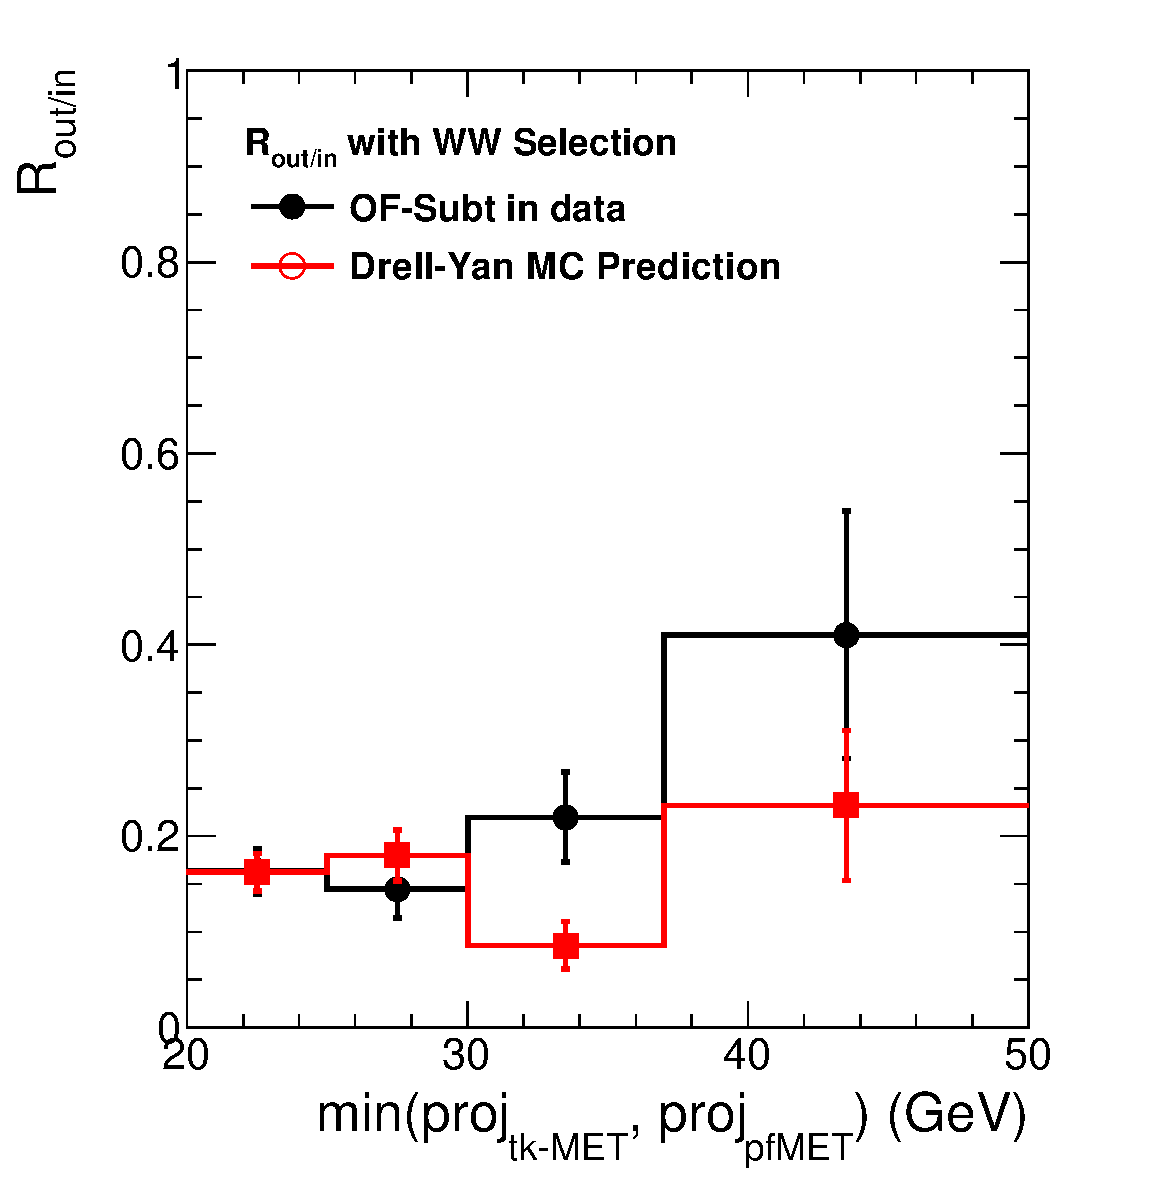
\includegraphics[width=.3\textwidth]{figures/Routin_ee_0Jet_mH0_4700pb_dy.pdf}}
\subfigure[mm]{
\centering
\label{subfig:dyr_mm_0j}
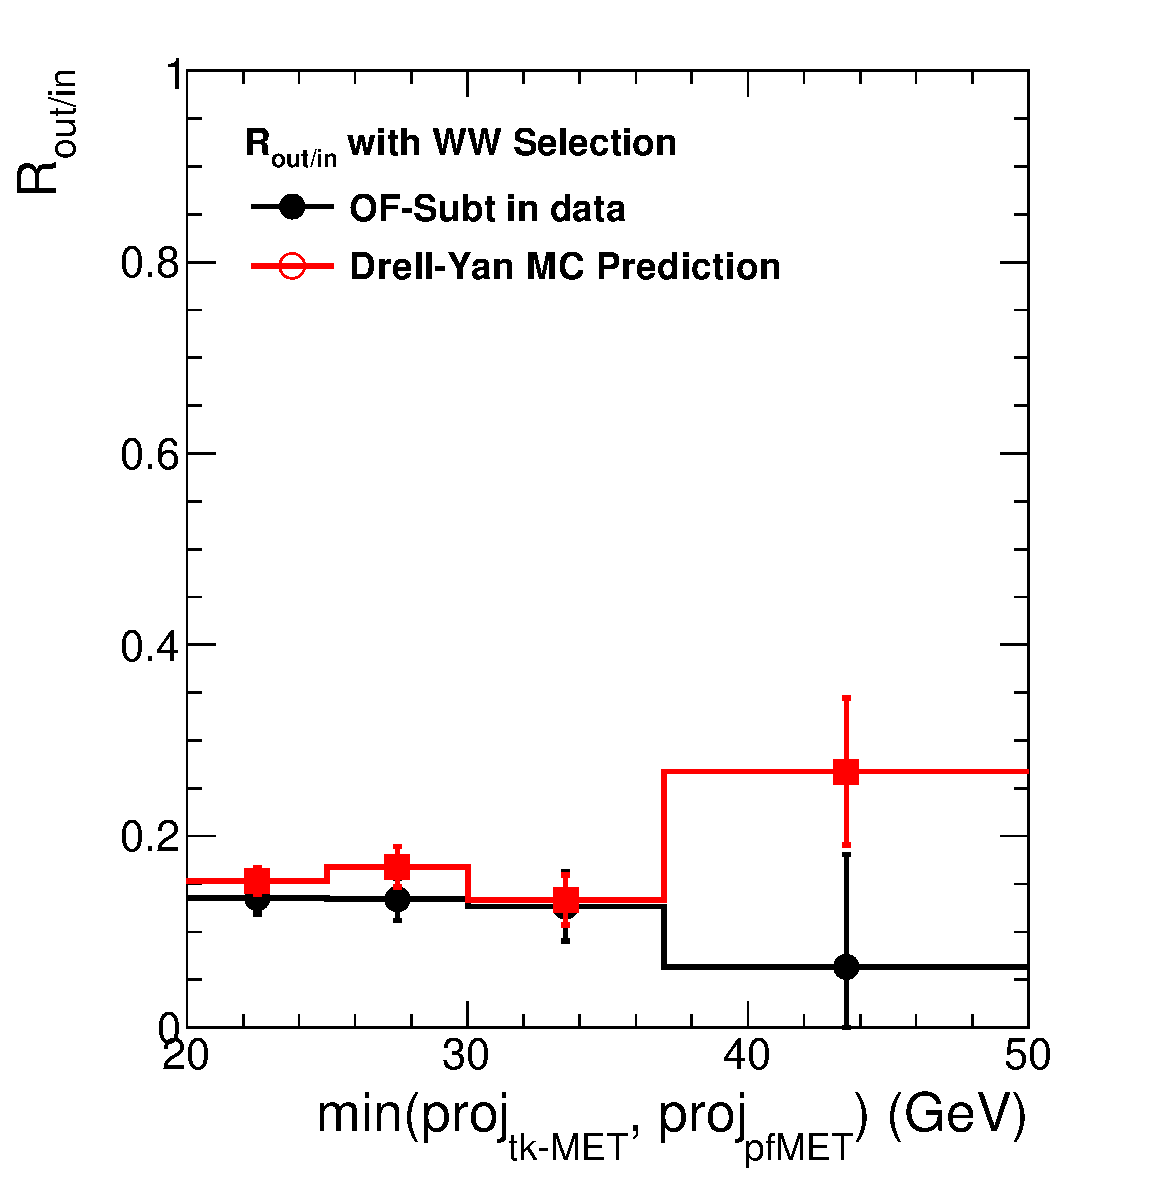
\includegraphics[width=.3\textwidth]{figures/Routin_mm_0Jet_mH0_4700pb_dy.pdf}}
\subfigure[ee/mm combined]{
\centering
\label{subfig:dyr_mm_0j}
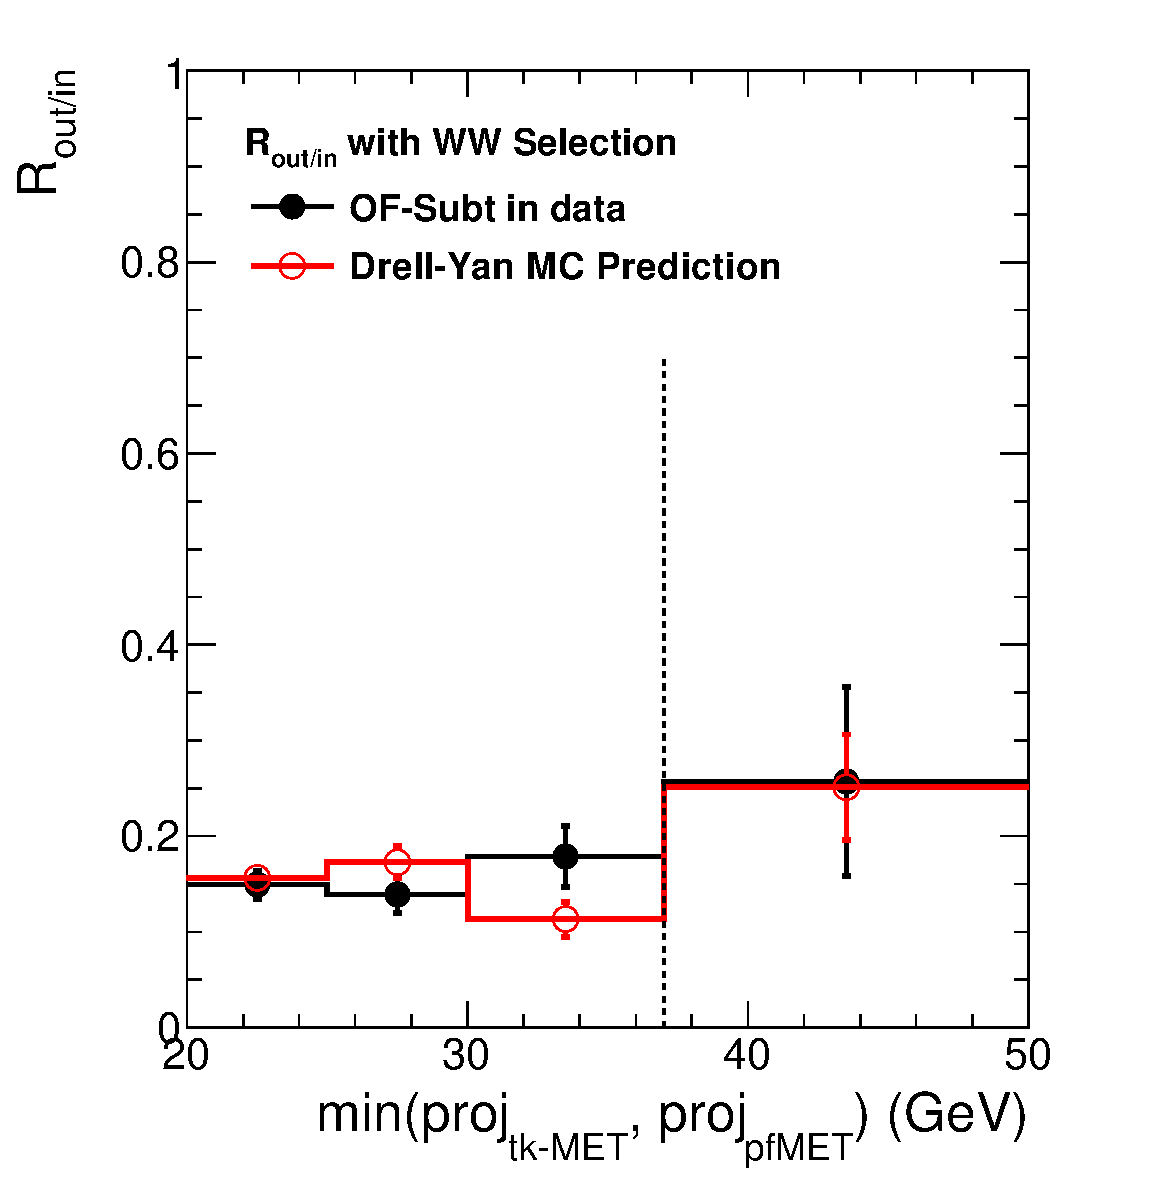
\includegraphics[width=.3\textwidth]{figures/Routin_0Jet_mH0_4700pb_dy.pdf}}
\caption{
 The \routin\, as a function of MET measured from data (black solid dots) 
and MC (red open circles) for the Drell-Yan processes. The measurements 
in data are done using the opposite flavor subtraction method. }
\label{fig:dyr_ww}
\end{figure}
%%%%%%%%%%%%%%%%%%%%%%

